\section{Modelamiento}

El modelo matemático se construyo en el software de análisis y diseño estructural ETABS en su versión 20.1.1, el material se definió según lo mencionado en el inciso 7 del presente documento, las secciones se crearon según lo mencionado en el predimensionamiento. Para el modelado de losas y muros se utilizo elementos shell y para columnas y vigas se utilizo elementos frame, sin embargo cuando existe columnas que forman parte de algún muro estos se modelaron con elementos shell para integrar de mejor manera los esfuerzos resultantes, asi mismo se aseguro un correcto mesh en esos elementos para poder capturar el comportamiento a flexion. 
\\
Las alturas de entrepiso se tomaron según los planos de arquitectura, la profundidad de cimentación se considero de 3.10m y las columnas y muros se modelaron hasta la cara superior de la cimentación, para lo cual se estimo un espesor de la zapata o platea de 0.6m. 
\\
Las zonas de los nudos de columnas y vigas se modelaron con un factor de rigidez del 50 \%, se consideran las rigideces brutas de los elementos como se menciona en la E-030 a excepción de las losas donde se redujo la rigidez axial, a flexión y a cortante a un 25 \% según lo mencionado en \cite{ACI19}. Debido a las aberturas y la relación de dimensiones de la planta del edificio no se considera un diafragma rígido en los sistemas de piso.
\\
\newpage

\newsavebox\mybox
\savebox{\mybox}{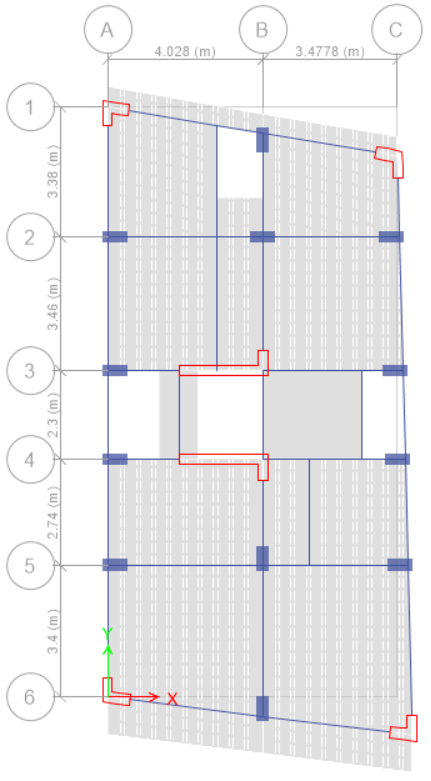
\includegraphics[width=7cm]{IMAGENES/6.PNG}}
\begin{figure}[h]
    \centering
    \begin{minipage}{0.45\textwidth}
        \centering
        \usebox{\mybox}
        \caption{Planta típica}
    \end{minipage}
    \begin{minipage}{0.45\textwidth}
        \centering
        \vbox to \ht\mybox{%
            \vfill
            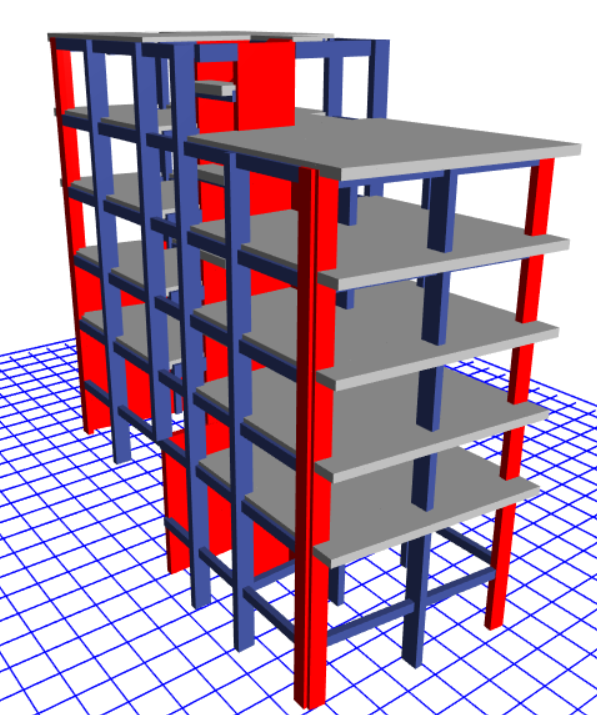
\includegraphics[width=7cm]{IMAGENES/5.PNG}
            \vfill
        }
        \caption{Vista 3D}
    \end{minipage}
\end{figure}